% ==============================================================================
% 第 4 章：区间、枚举与分类 (Chapter 4: Intervals, Enumerations, and Itemizations)
% ==============================================================================

\chapter{区间、枚举与分类}
\label{sec:ch04_intervals}

目前为止，你有四种将信息表示为数据的方式：数、字符串、图像与布尔值。对于许多简单问题，这四种基本类型已经足够；但在更多情况下，BSL（乃至任何编程语言）中这四种原始数据集合远远无法满足实际需求。真正的程序设计者需要更丰富的手段来将现实世界的信息表示为计算数据。

作为起步，优秀程序员必须学会对这些内置集合进行\term{约束与划分}。一种方法是从集合中明确\term{枚举}（enumerate）出一组离散的元素，并声明在此问题中只使用这些特定元素。显然，枚举仅适用于元素总数有限的情况。为了表示包含“无限”多个元素的集合，我们引入了\term{区间}（interval）——即满足某种特定数学属性的一组连续或离散的值。

\begin{notebox}[关于“无限”的说明]
这里的“无限”通常也可以指“规模大到对其逐一枚举在工程上完全不切实际”。
\end{notebox}

定义枚举与区间意味着我们需要对不同类型的数据进行区分。在代码中，区分不同的数据需要借助\term{条件函数}（conditional functions），即能够根据传入参数的具体取值选择不同计算路径的函数。在“多种计算方式”以及第 1.6 节中，我们已经见识过编写这类函数的示例。但当时的讨论并未涉及系统性的程序设计，而仅仅是在介绍 BSL 语言的新语法特性。

在本章中，我们将讨论适用于枚举与区间的通用设计方法。首先，我们重新审视 \code{cond} 条件表达式；接着依次探讨三种不同类型的数据描述方式：\term{枚举}（enumerations）、\term{区间}（intervals）和\term{分项数据 / 分类}（itemizations）。枚举会完整列出属于该集合的每一个数据元素；区间则指定一个连续或边界清晰的数据范围；而分类则将前两者融合在一起，在定义的某些分支中指定范围，在另一些分支中指定具体离散的数据。本章最后将归纳处理此类情况的通用设计配方，并探讨其在有限状态世界程序中的经典应用。

% ==============================================================================
\section{使用条件表达式编程}
\label{sec:4.1_programming_with_conditionals}
% ==============================================================================

回想我们在序幕中对条件表达式的简短介绍。由于 \code{cond} 是本书中涉及的最复杂表达式形式，让我们仔细观察其通用形式：

\begin{lstlisting}[language=BSL]
(cond
  [ConditionExpression_1 ResultExpression_1]
  [ConditionExpression_2 ResultExpression_2]
  ...
  [ConditionExpression_N ResultExpression_N])
\end{lstlisting}

\begin{notebox}[语法提示：方括号与圆括号]
方括号 \code{[...]} 的作用是让每个 \code{cond} 分支更加醒目。在 BSL 语法中，用普通圆括号 \code{(...)} 代替方括号也是完全合法的。
\end{notebox}

一个 \code{cond} 表达式以关键字 \code{(cond} 开头，并以匹配的 \code{)} 结尾。紧随关键字之后，程序员可以书写任意多个 \code{cond} 行（行数视需求而定）；每一行包含两个表达式，由左右方括号 \code{[} 与 \code{]} 包裹。

一个 \code{cond} 行在专业术语中在术语上被称为一个 \code{cond} \term{条件分支}（或\term{条件子句}，cond clause）。

下面是一个使用条件表达式的函数定义：

\begin{lstlisting}[language=BSL]
(define (next traffic-light-state)
  (cond
    [(string=? "red" traffic-light-state) "green"]
    [(string=? "green" traffic-light-state) "yellow"]
    [(string=? "yellow" traffic-light-state) "red"]))
\end{lstlisting}

就像序幕中的数学分段函数一样，这个例子展示了使用 \code{cond} 表达式的便利之处。在许多问题场景中，函数必须区分若干种互斥的情况。借助 \code{cond} 表达式，你可以为每种可能性分配单独的一行，从而直观地对应于问题描述中的各个分支。

\begin{notebox}[编程实践备忘：cond 与 if 的选择]
请对比 \code{cond} 表达式与第 1.6 节中的 \code{if} 表达式。\code{if} 表达式擅长将“一种情况与其余所有情况”区分开来（二选一）。因此，当面对多重情况时，嵌套的 \code{if} 会变得极其冗长且难以阅读。我们达成一个共识：只要分支直接源于数据定义中的多种情况，就一律使用 \code{cond}；只有在表达单纯的“非此即彼”二选一时，才使用 \code{if}。
\end{notebox}

当 \code{cond} 表达式中的条件判断变得繁琐时，你有时希望表达“在其余所有情况下”的兜底语义。为此，BSL 允许在 \code{cond} 表达式的\textbf{最后一行}使用关键字 \code{else}：

\begin{lstlisting}[language=BSL]
(cond
  [ConditionExpression_1 ResultExpression_1]
  [ConditionExpression_2 ResultExpression_2]
  ...
  [else DefaultResultExpression])
\end{lstlisting}

如果你误在其他位置使用了 \code{else}，DrRacket 会立即报错：

\begin{replbox}
> (cond
    [(> x 0) 10]
    [else 20]
    [(< x 10) 30])
cond: found an else clause that isn't the last clause in its cond expression
\end{replbox}

也就是说，BSL 严格拒绝在语法上无意义或歧义的结构。

假设我们要设计一个在游戏结束时计算奖励等级的函数。下面是该函数的签名与说明：

\begin{lstlisting}[language=BSL]
; PositiveNumber 代表非负数（即大于或等于 0 的数）
; PositiveNumber -> String
; 根据给定的得分 s 计算对应的奖励等级
\end{lstlisting}
\footnote{严格在数学上，大于或等于 0 的数称为“非负数”（Non-negative Number），严格大于 0 的数才称为“正数”（Positive Number）。原书在此处为了降低初学者门槛，宽松地使用了 \code{PositiveNumber} 作为类型名来指代 $[0, \infty)$ 区间。本书在代码中沿用原书标识符以保持与练习和测试用例一致，正文表述中统一明确其非负数含义。}

下面给出两种对比实现：

\begin{figure}[htbp]
  \centering
  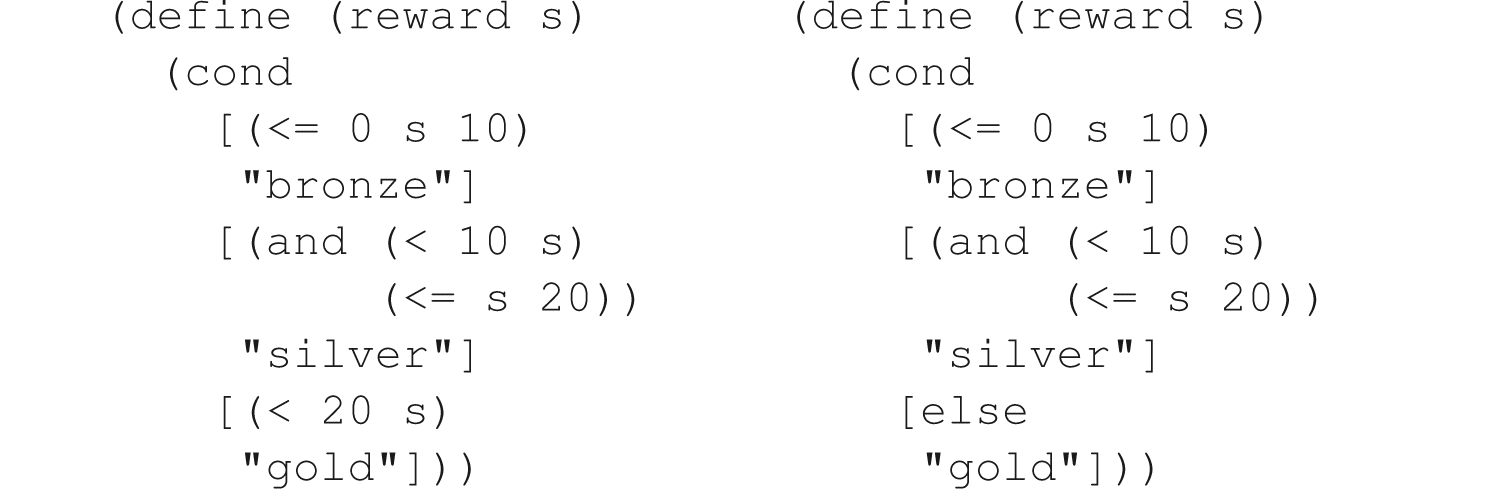
\includegraphics[width=0.85\textwidth]{images/00071.png}
  \caption{显式全条件（左）与使用 else 分支（右）的对比}
  \label{fig:reward_compare}
\end{figure}

左侧变体使用了包含三个完整布尔条件的 \code{cond}；而右侧则在末尾使用了 \code{else} 分支。为了推导左侧第三个条件 \code{(< 20 s)}，你必须在头脑中计算推断出：
\begin{itemize}
  \item $s$ 是一个 \code{PositiveNumber}（即非负数）；
  \item \code{(<= 0 s 10)} 的求值结果为 \code{\#false}；
  \item \code{(and (< 10 s) (<= s 20))} 的求值结果同样为 \code{\#false}。
\end{itemize}

尽管在这个简单例子中心算并不复杂，但当业务规则变得交错时，手动推导互补条件极易出错并埋下隐患。因此，当你明确需要对前述所有条件取反（即逻辑上的\term{补集}，complement）时，使用右侧带有 \code{else} 的写法更为稳妥清晰。

\begin{exercise}{单步调试奖励函数}{48}
将 \code{reward} 的函数定义以及测试调用 \code{(reward 18)} 键入 DrRacket 的定义区，并点击“单步求值器”（Stepper），观察 DrRacket 是如何一步步对函数应用进行求值的。
\end{exercise}

\begin{exercise}{嵌套条件表达式}{49}
\code{cond} 本身就是一个表达式，因此它完全可以嵌套在另一个表达式内部。例如：
\begin{lstlisting}[language=BSL]
(- 200 (cond [(> y 200) 0] [else y]))
\end{lstlisting}

请参考图~\ref{fig:ch04_rocket_recall} 中的 \code{create-rocket-scene.v5} 函数，重构该函数并使用嵌套的 \code{cond} 表达式，使得新函数体中仅出现一次 \code{place-image} 调用。

\begin{center}
  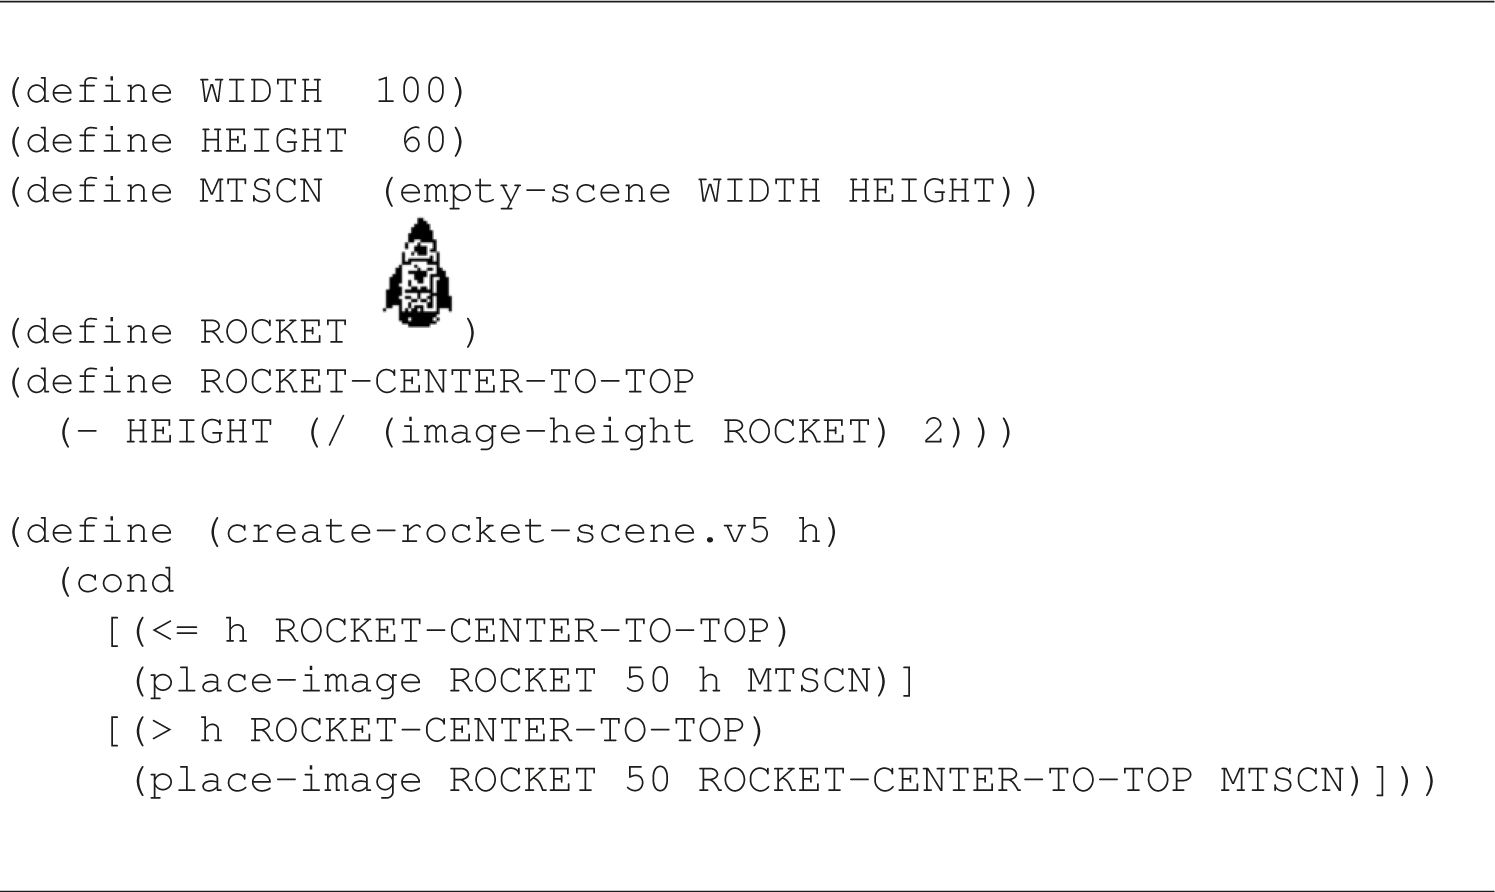
\includegraphics[width=0.75\textwidth]{images/00072.jpeg}
  \captionof{figure}{火箭发射场景生成函数}\label{fig:ch04_rocket_recall}
\end{center}
\end{exercise}

% ==============================================================================
\section{条件计算过程}
\label{sec:4.2_computing_conditionally}
% ==============================================================================

理解条件表达式的核心在于掌握其严格的求值规则。其计算归约（reduction）过程遵循以下规则：

\begin{notebox}[cond 表达式的求值规则]
对于形如 \code{(cond [C\_1 R\_1] [C\_2 R\_2] ...)} 的表达式：
\begin{enumerate}
  \item DrRacket 从上到下依次对条件表达式 $C_i$ 求值。
  \item 若 $C_1$ 求值结果为 \code{\#true}，则整个 \code{cond} 表达式立刻被替换为其对应的结果表达式 $R_1$。
  \item 若 $C_1$ 求值结果为 \code{\#false}，则该条件分支被完全丢弃，计算继续对剩下的分支进行。
  \item 若 $C_1$ 的求值结果既非 \code{\#true} 亦非 \code{\#false}，BSL 报错：\code{cond: question result is not true or false}。
  \item 若遭遇 \code{[else R]}，它无条件等价于 \code{\#true}，整个表达式直接被替换为 $R$。
  \item 若所有条件均为 \code{\#false} 且没有 \code{else} 分支，BSL 报错：\code{cond: all question results were false}。
\end{enumerate}
\end{notebox}

让我们以 \code{(reward 3)} 的计算为例进行单步追踪：
\begin{lstlisting}[language=BSL]
  (reward 3)
== (cond
     [(<= 0 3 10) "bronze"]
     [(and (< 10 3) (<= 3 20)) "silver"]
     [else "gold"])
== (cond
     [#true "bronze"]
     [(and (< 10 3) (<= 3 20)) "silver"]
     [else "gold"])
== "bronze"
\end{lstlisting}

再看当输入为 21 时的情况：
\begin{lstlisting}[language=BSL]
  (reward 21)
== (cond
     [(<= 0 21 10) "bronze"]
     [(and (< 10 21) (<= 21 20)) "silver"]
     [else "gold"])
== (cond
     [#false "bronze"]
     [(and (< 10 21) (<= 21 20)) "silver"]
     [else "gold"])
== (cond
     [(and (< 10 21) (<= 21 20)) "silver"]
     [else "gold"])
== (cond
     [(and #true (<= 21 20)) "silver"]
     [else "gold"])
== (cond
     [(and #true #false) "silver"]
     [else "gold"])
== (cond
     [#false "silver"]
     [else "gold"])
== (cond
     [else "gold"])
== "gold"
\end{lstlisting}

\begin{exercise}{测试覆盖度}{50}
如果你将本章第一节的 \code{next} 函数复制到 DrRacket 定义区并点击“Run”，DrRacket 会高亮显示三行 \code{cond} 中的两行（颜色通常为黑色背景加亮）。这种高亮表示你的测试用例未能覆盖所有的条件分支。请补充足够的测试用例，使测试覆盖所有情况。
\end{exercise}

\begin{exercise}{模拟红绿灯世界程序}{51}
设计一个使用 \code{big-bang} 的世界程序，在指定的时间跨度内模拟交通信号灯的状态变迁。程序将信号灯的状态渲染为一个填充了对应颜色的实心圆，并且在每个时钟滴答（clock tick）发生时改变颜色。哪种颜色是最合适的初始状态？不妨咨询一下工程专业的朋友。
\end{exercise}

% ==============================================================================
\section{枚举}
\label{sec:4.3_enumerations}
% ==============================================================================

在程序设计中，当现实中的状态仅存在有限个离散可能时，我们使用\term{枚举}（Enumeration）来定义数据。

\begin{lstlisting}[language=BSL]
; 一个 TrafficLight 是以下三者之一：
; -- "red"
; -- "green"
; -- "yellow"
; 解释：交通信号灯的三种法定显示颜色
\end{lstlisting}

数据定义的核心目的在于：向读者明确指出该集合包含哪些值，以及这些值在现实世界中对应什么物理含义。在枚举中，我们逐一列出属于该集合的所有合法值。

除了自定义枚举，BSL 还提供了若干内置的大型枚举，最典型的便是按键事件 \code{KeyEvent} 和鼠标事件 \code{MouseEvent}。一个 \code{KeyEvent} 本质上是一个包含上百个合法字符串的枚举（如 \code{"a"}, \code{"b"}, \code{"left"}, \code{"right"}, \code{"\ "} 等）。

\begin{figure}[htbp]
  \centering
  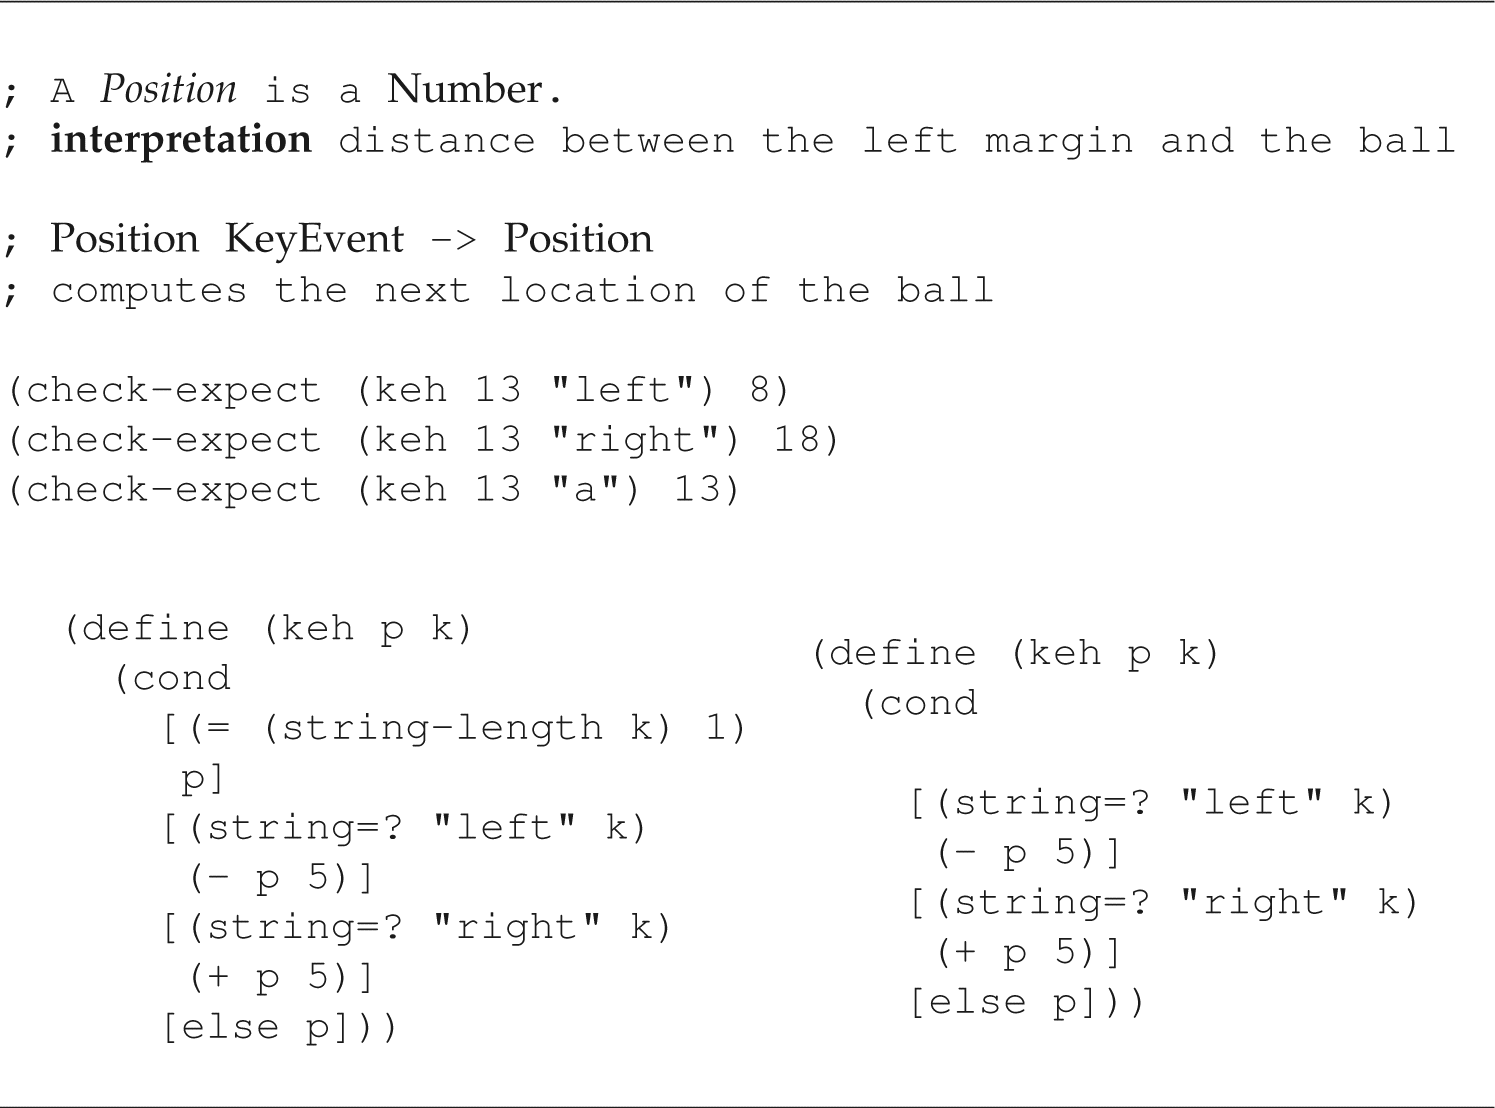
\includegraphics[width=0.9\textwidth]{images/00073.png}
  \caption{条件函数与特殊枚举处理的两种方式}
  \label{fig:deal_with_keys_compare}
\end{figure}

图~\ref{fig:deal_with_keys_compare} 展示了处理枚举的两种思路。左侧遵循“数据定义的每一项对应 \code{cond} 的一行”的标准规范；右侧则针对特殊场景进行了精简重组：将我们关心的两颗方向键单独处理，其他所有未关心的按键统统归入 \code{else}。这种代码重构通常应当在按照设计配方完成基础设计之后再审慎进行。

% ==============================================================================
\section{区间}
\label{sec:4.4_intervals}
% ==============================================================================

当可能的数据量非常庞大或连续时，枚举就无能为力了。此时我们使用\term{区间}（Interval）来圈定数据范围。

数学上，我们使用开区间与闭区间的符号体系：
\begin{itemize}
  \item $[a, b]$ 表示包含两端点的闭区间：$\{x \in \mathbb{R} \mid a \le x \le b\}$；
  \item $(a, b)$ 表示不包含两端点的开区间：$\{x \in \mathbb{R} \mid a < x < b\}$；
  \item $[a, b)$ 和 $(a, b]$ 分别表示半开半闭区间；
  \item $[a, \infty)$ 表示无上界的右向无穷区间：$\{x \in \mathbb{R} \mid x \ge a\}$。
\end{itemize}

在数据定义中，我们可以清晰地书写区间：
\begin{lstlisting}[language=BSL]
; A PositiveNumber is a Number greater than/equal to 0.
; 一个非负数（原书类型名作 PositiveNumber）是大于或等于 0 的数：[0, \infty)
\end{lstlisting}

\begin{figure}[htbp]
  \centering
  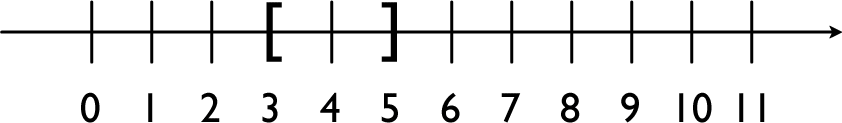
\includegraphics[width=0.6\textwidth]{images/00075.png}\\[1ex]
  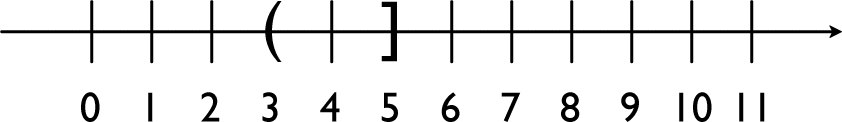
\includegraphics[width=0.6\textwidth]{images/00076.png}\\[1ex]
  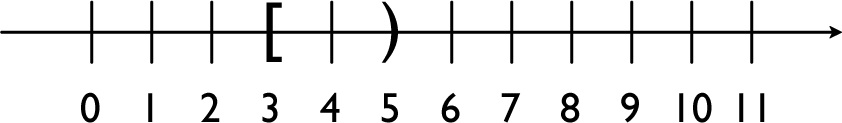
\includegraphics[width=0.6\textwidth]{images/00077.png}\\[1ex]
  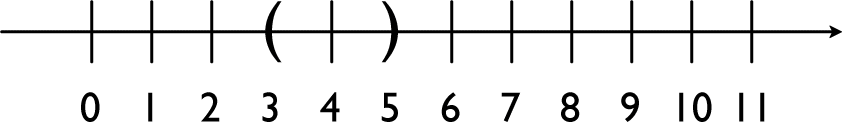
\includegraphics[width=0.6\textwidth]{images/00078.png}\\[1ex]
  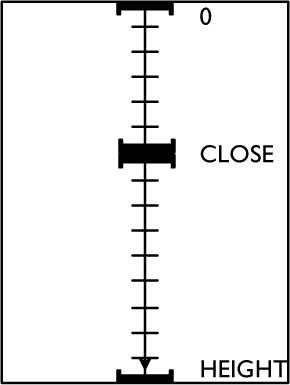
\includegraphics[width=0.6\textwidth]{images/00079.png}
  \caption{各类型区间的数轴可视化}
  \label{fig:number_lines}
\end{figure}

数轴可视化（图~\ref{fig:number_lines}）在两方面极大地指导了函数设计：
\begin{enumerate}
  \item 它直观指引了\textbf{测试用例的选取}：我们不仅需要在区间的“内部”挑选典型点，还必须精确选取区间的“端点”（边界条件），因为边界是最容易出现 $\le$ 与 $<$ 混淆的地方。
  \item 它明确了\textbf{条件判断的公式}：例如判定一个数 $x$ 是否位于 $[3, 5]$ 内，条件表达式应写作 \code{(<= 3 x 5)}。
\end{enumerate}

\begin{exercise}{区间整数判定}{52}
观察上述四幅数轴图，分别指出各个区间内包含哪些整数？
\end{exercise}

\subsection{案例研究：UFO 降落程序}

让我们考虑一个 UFO 从天空中降落的交互式程序。
如图~\ref{fig:ufo_descending} 所示，我们首先确立基础常数与数据定义：

\begin{figure}[htbp]
  \centering
  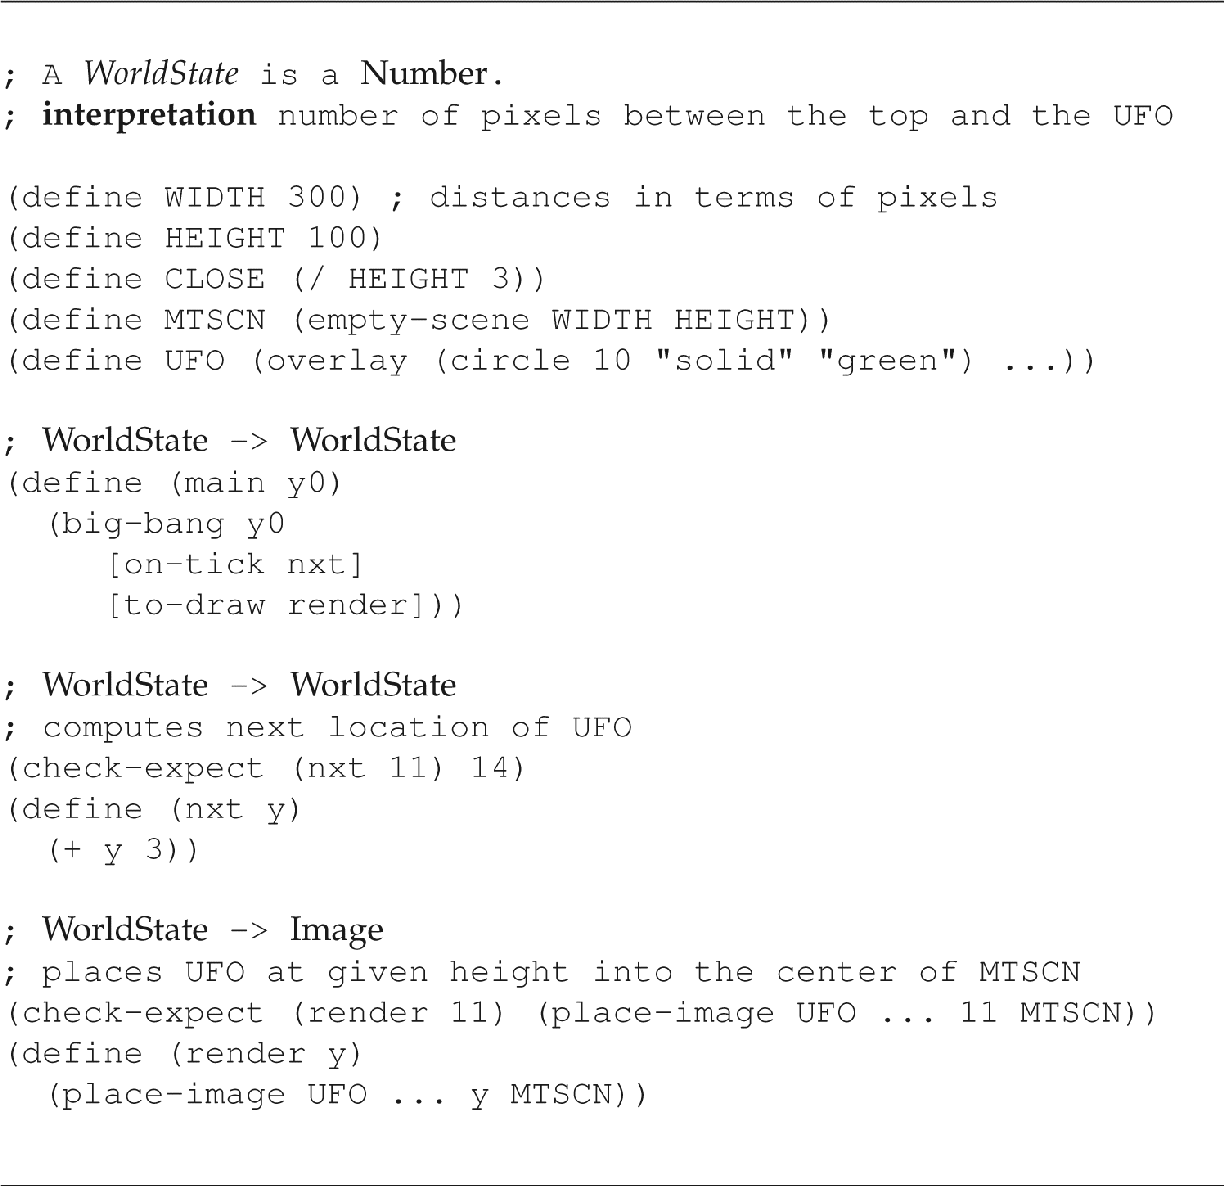
\includegraphics[width=0.85\textwidth]{images/00074.png}
  \caption{UFO 降落的世界程序骨架}
  \label{fig:ufo_descending}
\end{figure}

\begin{lstlisting}[language=BSL]
(define WIDTH 300)
(define HEIGHT 100)
(define CLOSE (/ HEIGHT 3))
(define MTSCN (empty-scene WIDTH HEIGHT))
(define UFO (overlay (circle 10 "solid" "green")
                     (rectangle 40 4 "solid" "green")))

; 一个 WorldState 是一个非负数 Number
; 解释：UFO 中心距离顶部的像素高度
\end{lstlisting}

现在我们希望为画面添加状态文本行：
\begin{itemize}
  \item 当 $0 \le y \le \text{CLOSE}$ 时，处于“降落中”（descending，显示为绿色）；
  \item 当 $\text{CLOSE} < y \le \text{HEIGHT}$ 时，处于“接近地面”（closing in，显示为橙色）；
  \item 当 $y > \text{HEIGHT}$ 时，处于“已着陆”（landed，显示为红色）。
\end{itemize}

\begin{figure}[htbp]
  \centering
  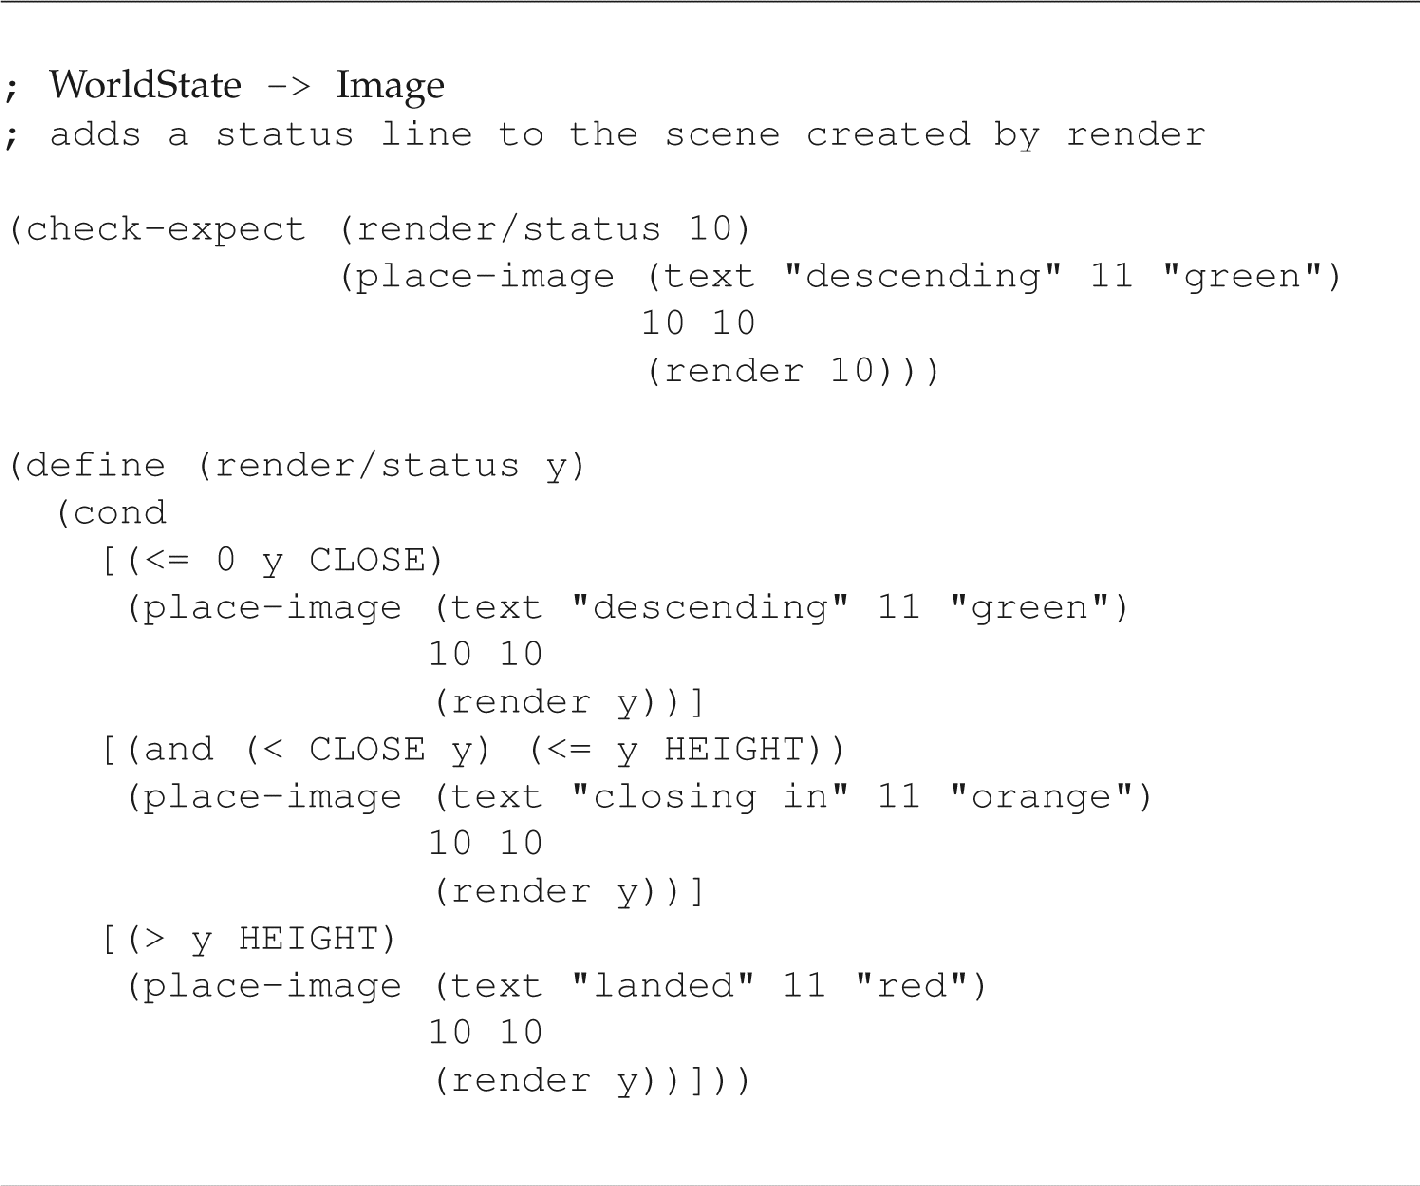
\includegraphics[width=0.85\textwidth]{images/00082.png}
  \caption{带有状态提示栏的渲染函数 render/status}
  \label{fig:render_status_orig}
\end{figure}

图~\ref{fig:render_status_orig} 给出了初版 \code{render/status} 的完整定义。观察该定义，三个分支中均出现了重复的渲染框架。通过将 \code{cond} 表达式嵌套在 \code{text} 的参数中，我们可以将其优雅地重构为图~\ref{fig:render_status_revised} 所示的形式。

\begin{figure}[htbp]
  \centering
  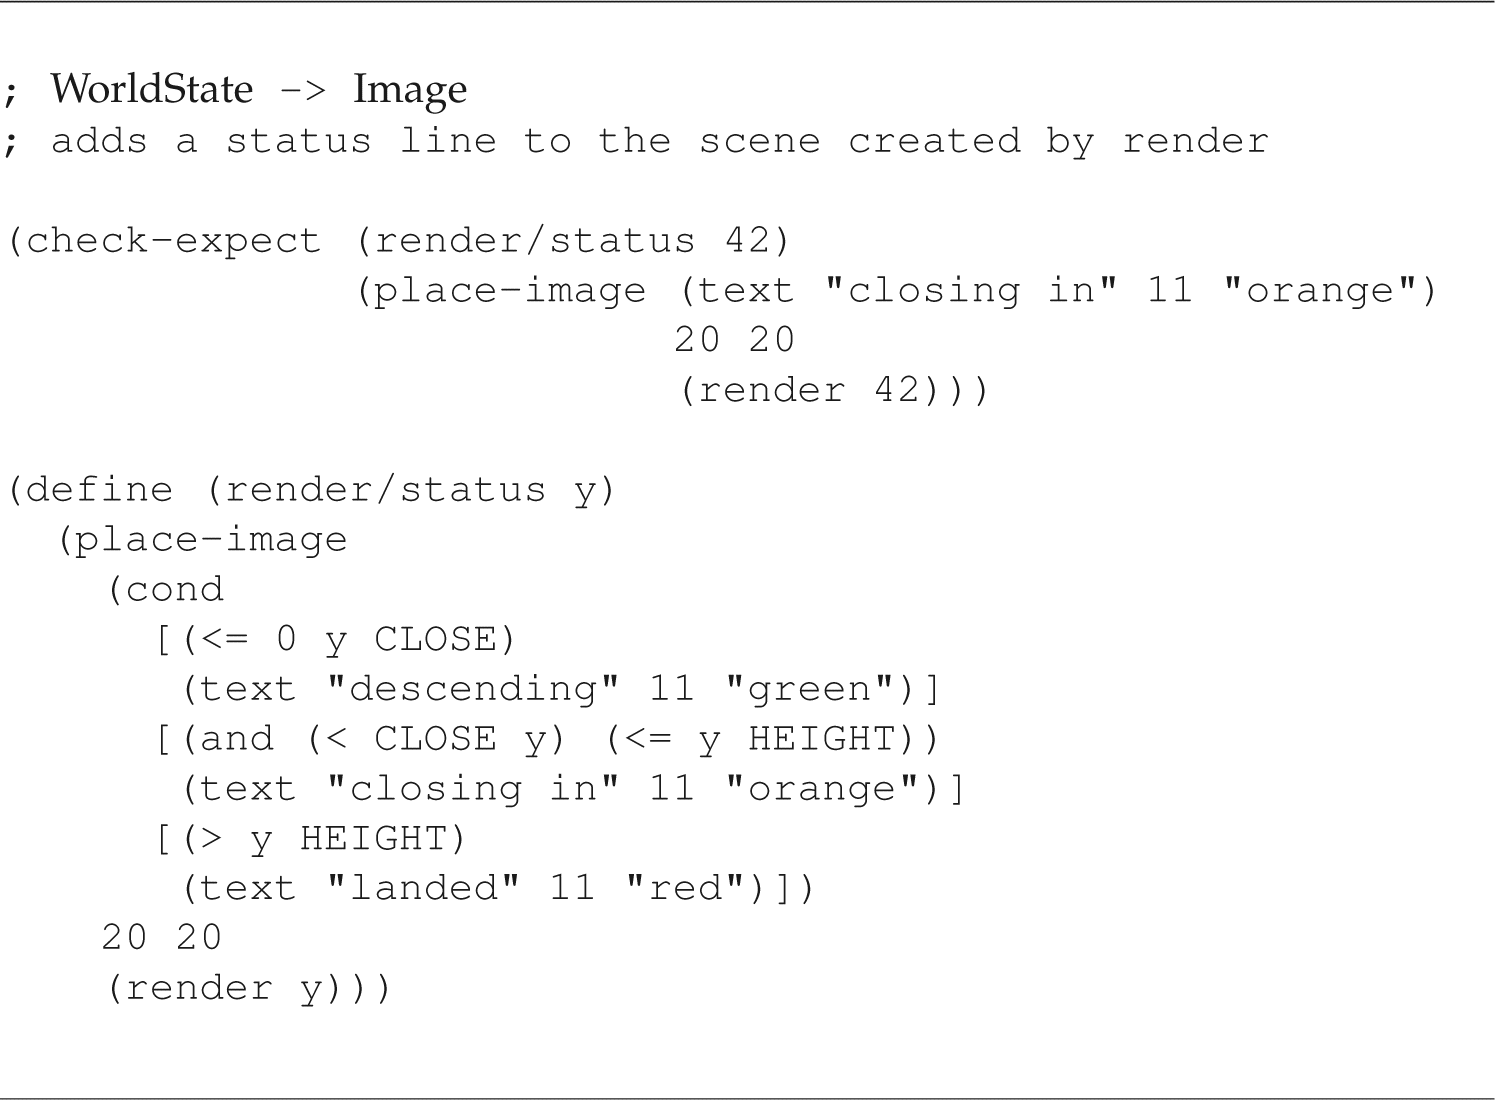
\includegraphics[width=0.85\textwidth]{images/00084.png}
  \caption{重构后的 render/status 函数}
  \label{fig:render_status_revised}
\end{figure}

% ==============================================================================
\section{分类 / 分项数据}
\label{sec:4.5_itemizations}
% ==============================================================================

在更复杂的世界中，一个状态量可能既包含区间，又包含若干特殊的离散标记。这种将不同性质的数据集合进行并集组合的数据描述称为\term{分类}或\term{分项数据}（Itemization）。

考虑一个火箭发射倒计时的世界程序。火箭在发射前处于静止状态，接着进行倒数（$-3, -2, -1$），最后点火升空并不断增加高度。我们可以将世界状态定义为：

\begin{lstlisting}[language=BSL]
; 一个 LRCD (火箭发射与倒计时状态) 是以下三者之一：
; -- "resting"
; -- 处于 [-3, -1] 之间的整数
; -- 一个非负数 NonNegativeNumber
; 解释：
; "resting" 表示火箭静止在发射架上；
; 负数代表发射前的倒计时秒数；
; 非负数代表火箭升空后距离地面的高度。
\end{lstlisting}

\begin{figure}[htbp]
  \centering
  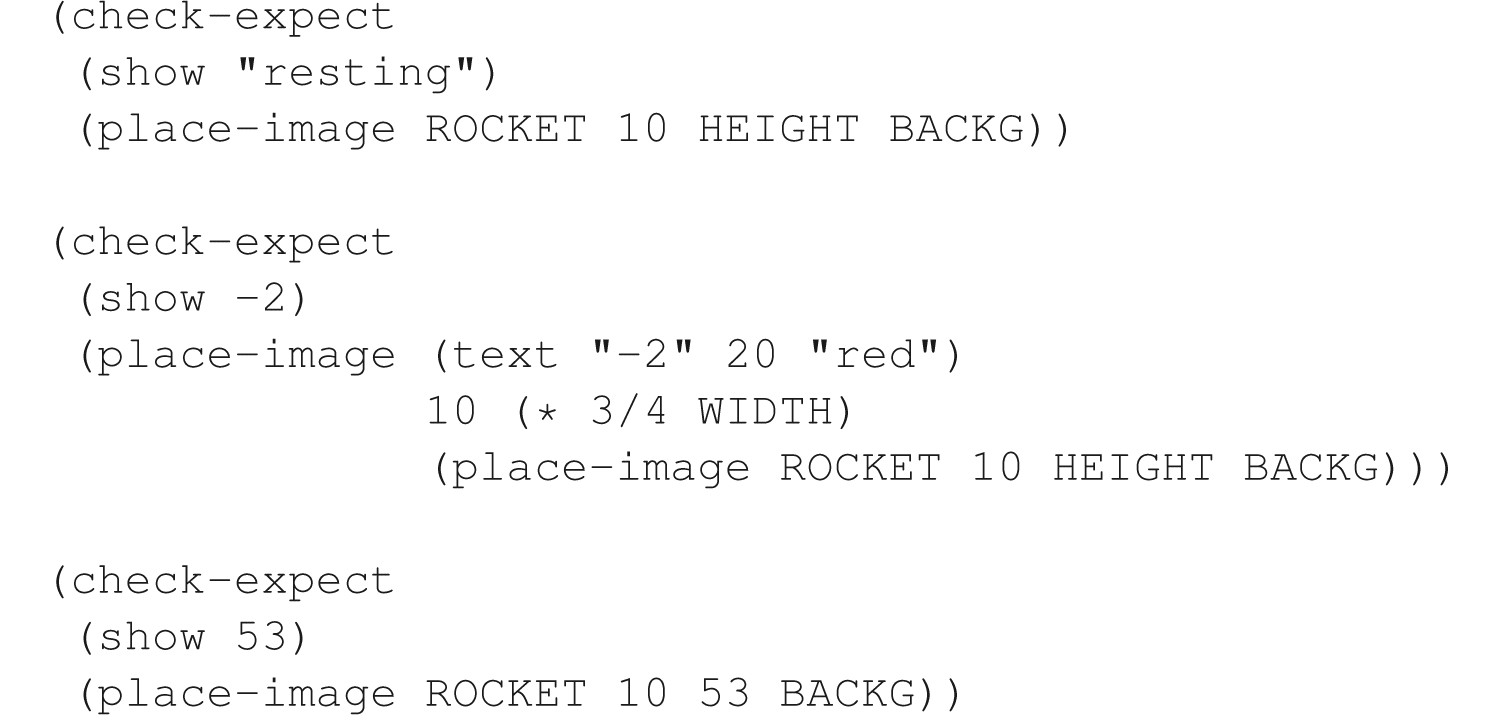
\includegraphics[width=0.7\textwidth]{images/00085.png}
  \caption{LRCD 状态的视觉示意图}
  \label{fig:lrcd_scenes}
\end{figure}

\begin{figure}[htbp]
  \centering
  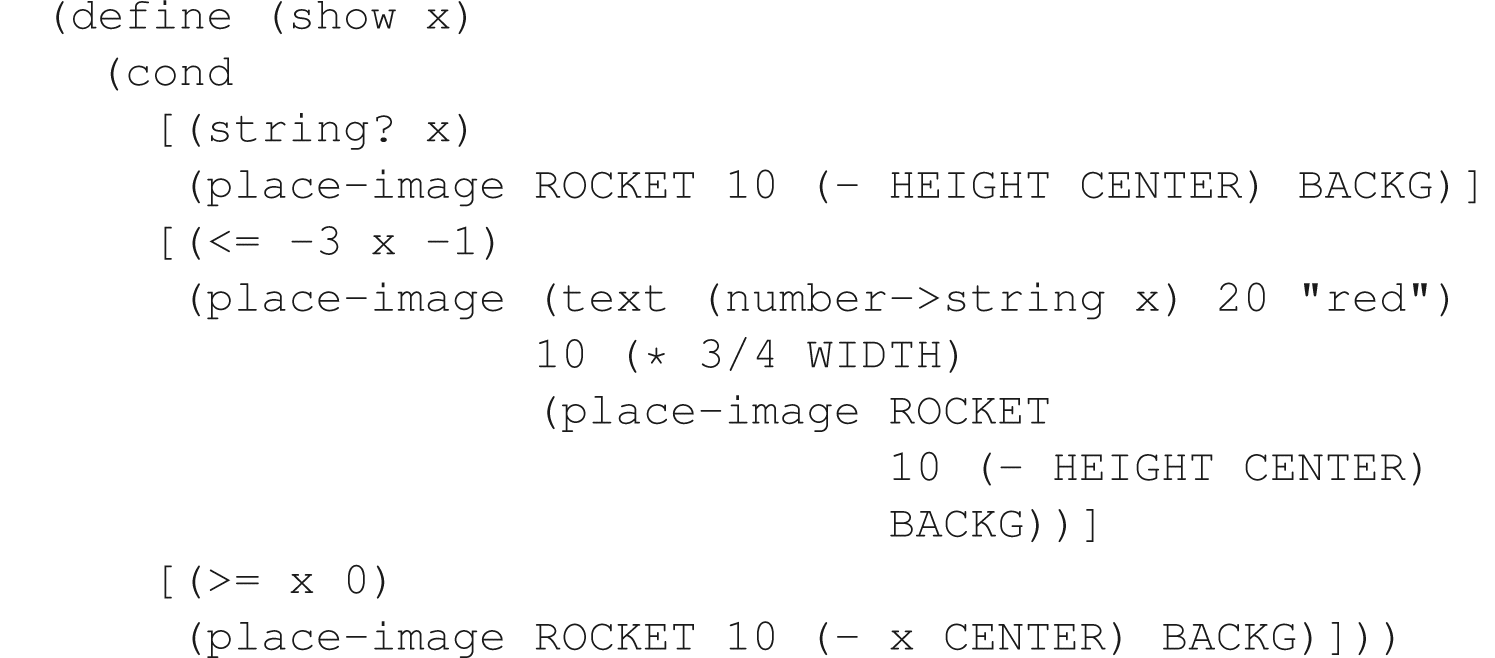
\includegraphics[width=0.8\textwidth]{images/00086.png}
  \caption{针对分类数据 LRCD 的函数模板骨架}
  \label{fig:lrcd_template}
\end{figure}

在图~\ref{fig:lrcd_template} 中，每一个分支条件严格对应数据定义的一个子类别。特别需要注意：在判定 \code{"resting"} 时，不能直接使用 \code{(string=? "resting" x)}，因为当参数 $x$ 为数时，\code{string=?} 会引发类型错误！必须使用更加安全的谓词或组合判断。

图~\ref{fig:ch04_rocket_full} 给出了该程序的各个关键事件处理函数的完整设计。

\begin{figure}[htbp]
  \centering
  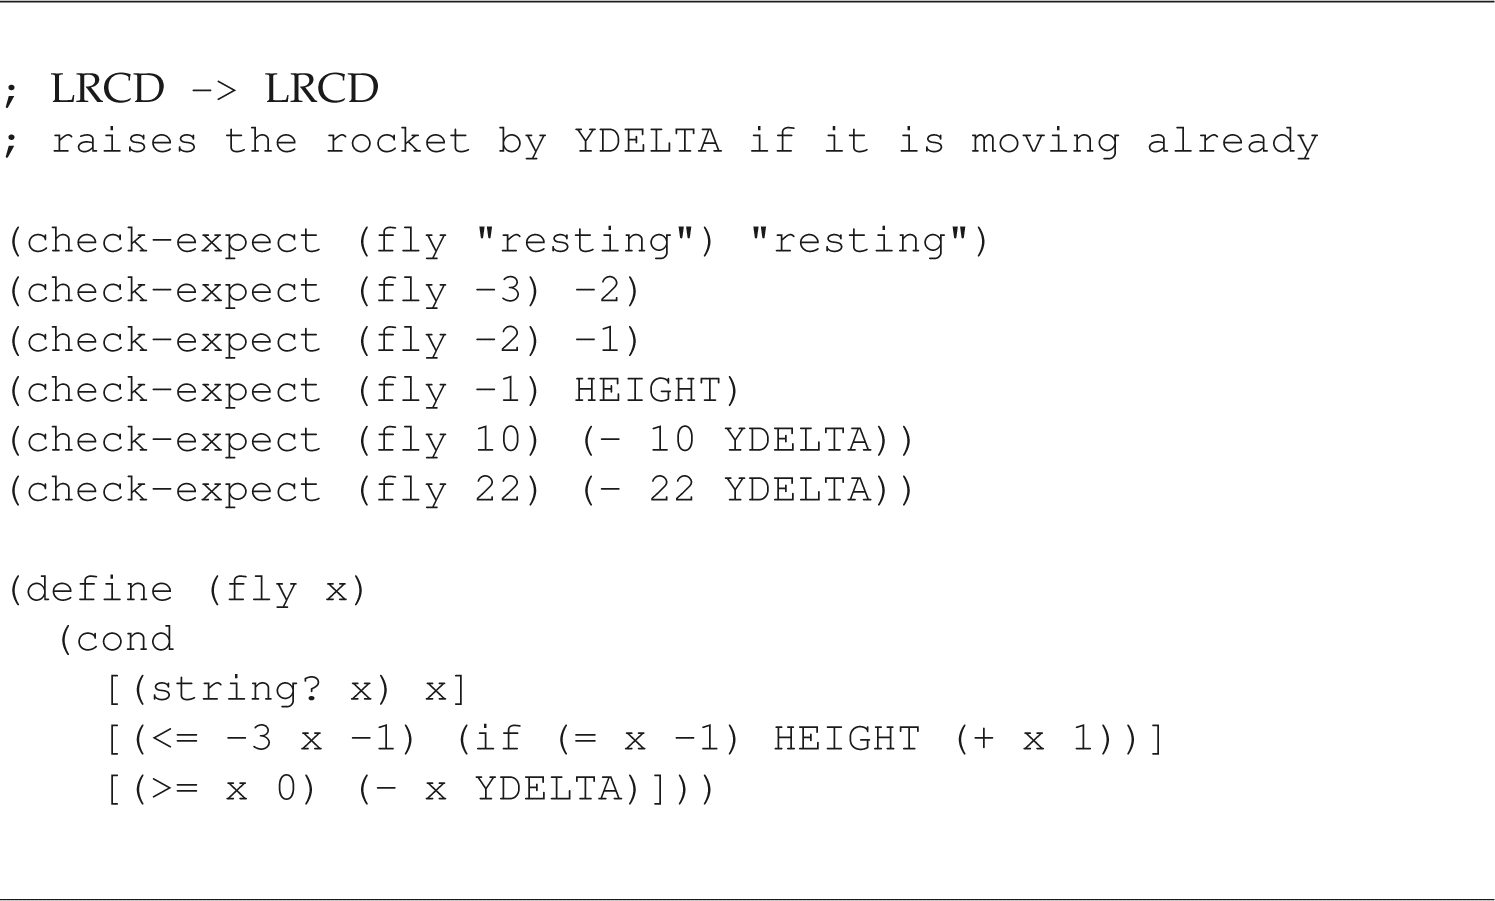
\includegraphics[width=0.9\textwidth]{images/00087.png}
  \caption{火箭发射倒计时程序的完整代码}
  \label{fig:ch04_rocket_full}
\end{figure}

\begin{exercise}{信息与数据的互转}{53}
世界程序的设计配方要求程序员能够在“现实信息”与“程序数据”之间自如转换。请根据 LRCD 的定义，绘制若干代表不同世界场景的草图，并写出对应的数据表示；反过来，选取至少包含 $0$ 和 \code{HEIGHT} 在内的几个数据样例，绘制其对应的场景图像。
\end{exercise}

\begin{exercise}{精确的条件谓词}{54}
为什么在 \code{show} 函数中将第一个条件写为 \code{(string=? "resting" x)} 是错误的？请写出一个完全严谨的条件表达式，使得它在且仅在 $x$ 属于 LRCD 的第一个子类时求值为 \code{\#true}。
\end{exercise}

\begin{exercise}{提取公共辅助函数}{55}
重新审视 \code{show} 函数。它包含了三处大致形如 \code{(place-image ROCKET 10 ... BACKG)} 的绘制逻辑。请设计一个辅助函数简化这些重复代码。
\end{exercise}

\begin{exercise}{完整的发射主程序}{56}
定义 \code{main2} 函数，使你能够按下空格键启动倒计时并亲眼目睹火箭升空。查阅 \code{on-tick} 子句的文档，了解一个滴答的默认时长以及如何自定义时钟频率。
\end{exercise}

\begin{exercise}{高度的另一种几何诠释}{57}
在物理学和计算机图形学中，“高度”可以有两种理解：距离地面的高度（自底向上）或在画布中的坐标（自顶向下）。重做本节的练习，改用另一种诠释方式，并对比两套方案的异同。
\end{exercise}

% ==============================================================================
\section{针对分类数据的设计}
\label{sec:4.6_designing_with_itemizations}
% ==============================================================================

现在我们提炼出针对\term{分类数据}（Itemization）的通用设计配方：

\begin{recipebox}{设计针对分类数据的函数}
\begin{enumerate}
  \item \textbf{数据定义}：明确列出所有互斥的子类（分支）。每个子类可以是具体的值、一个枚举、一个区间或甚至另一个类型。
  \item \textbf{签名、目的说明与函数头}：根据数据定义确定输入输出类型，简述函数计算逻辑，列出形参名。
  \item \textbf{功能示例}：\textbf{为每个子类至少设计一个典型示例}！对于包含区间的子类，必须在区间内部选取测试点，并在区间所有端点（边界）处各选取一个测试点。
  \item \textbf{函数模板}：
    \begin{itemize}
      \item 根据数据定义中子类的个数，写出包含同样数量分支的 \code{cond} 表达式；
      \item 为每个分支构思严密且互斥的条件判定表达式（Condition Expressions）；
      \item 留出结果表达式占位符 \code{...}。
    \end{itemize}
  \item \textbf{函数体实现}：针对每一个分支，结合该分支所承诺的数据特质，补全对应的计算结果表达式。
  \item \textbf{测试与验证}：将第 3 步中的功能示例全部转化为 \code{check-expect} 自动化测试，确保测试用例覆盖代码中的每一个分支。
\end{enumerate}
\end{recipebox}

\begin{table}[htbp]
  \centering
  \caption{不同价格对应的消费税初算示例}
  \label{tab:tax_examples}
  \small
  \setlength{\tabcolsep}{6pt}
  \begin{tabular}{lcccccc}
    \hline
    价格 & 0 & 537 & 1000 & 1282 & 10000 & 12017 \\
    \hline
    税额 & 0 & 0 & ???? & 64 & ????? & 961 \\
    \hline
  \end{tabular}
\end{table}

\subsection{案例：税收王国的分段税率函数}

在虚构的“税收之国”（Tax Land），消费税采用累进阶梯制：
\begin{itemize}
  \item 价格低于 1000 元：免税（税率 0\%）；
  \item 价格在 1000 到 10000 元之间：税率 5\%；
  \item 价格达到 10000 元及以上：奢侈品税率 8\%。
\end{itemize}

我们遵循设计配方：

\begin{lstlisting}[language=BSL]
; 1. 数据定义
; 一个 Price 是大于或等于 0 的数。
; 一个 TaxLandPrice 是以下三者之一：
; -- [0, 1000) 区间内的数，表示低价商品
; -- [1000, 10000) 区间内的数，表示普通商品
; -- [10000, \infty) 区间内的数，表示奢侈品

; 2. 签名、目的说明与函数头
; Price -> Number
; 计算给定价格 p 所需缴纳的消费税
(define (tax p) 0)

; 3. 功能示例与边界点
(check-expect (tax 0) 0)
(check-expect (tax 500) 0)
(check-expect (tax 1000) (* 0.05 1000))
(check-expect (tax 5000) (* 0.05 5000))
(check-expect (tax 10000) (* 0.08 10000))
(check-expect (tax 12000) (* 0.08 12000))

; 4. 函数模板
; (define (tax p)
;   (cond
;     [(< p 1000) ...]
;     [(and (<= 1000 p) (< p 10000)) ...]
;     [(>= p 10000) ...]))

; 5. 函数体实现
(define (tax p)
  (cond
    [(< p 1000) 0]
    [(and (<= 1000 p) (< p 10000)) (* 0.05 p)]
    [else (* 0.08 p)]))
\end{lstlisting}

\begin{exercise}{税收阶梯常数化}{58}
引入常量定义，将免税额度阈值与奢侈品门槛定义为常量，以便税收王国的议会能够随时轻松上调税率阈值。
\end{exercise}

% ==============================================================================
\section{有限状态世界}
\label{sec:4.7_finite_state_worlds}
% ==============================================================================

很多互动式程序可以被建模为\term{有限状态机}（Finite State Automaton, FSA）：系统在任意时刻必定处于有限个状态中的某一个，外部事件（如按键、时钟滴答）会触发系统从当前状态转移（transition）到另一个状态。

\subsection{交通信号灯状态机}

\begin{figure}[htbp]
  \centering
  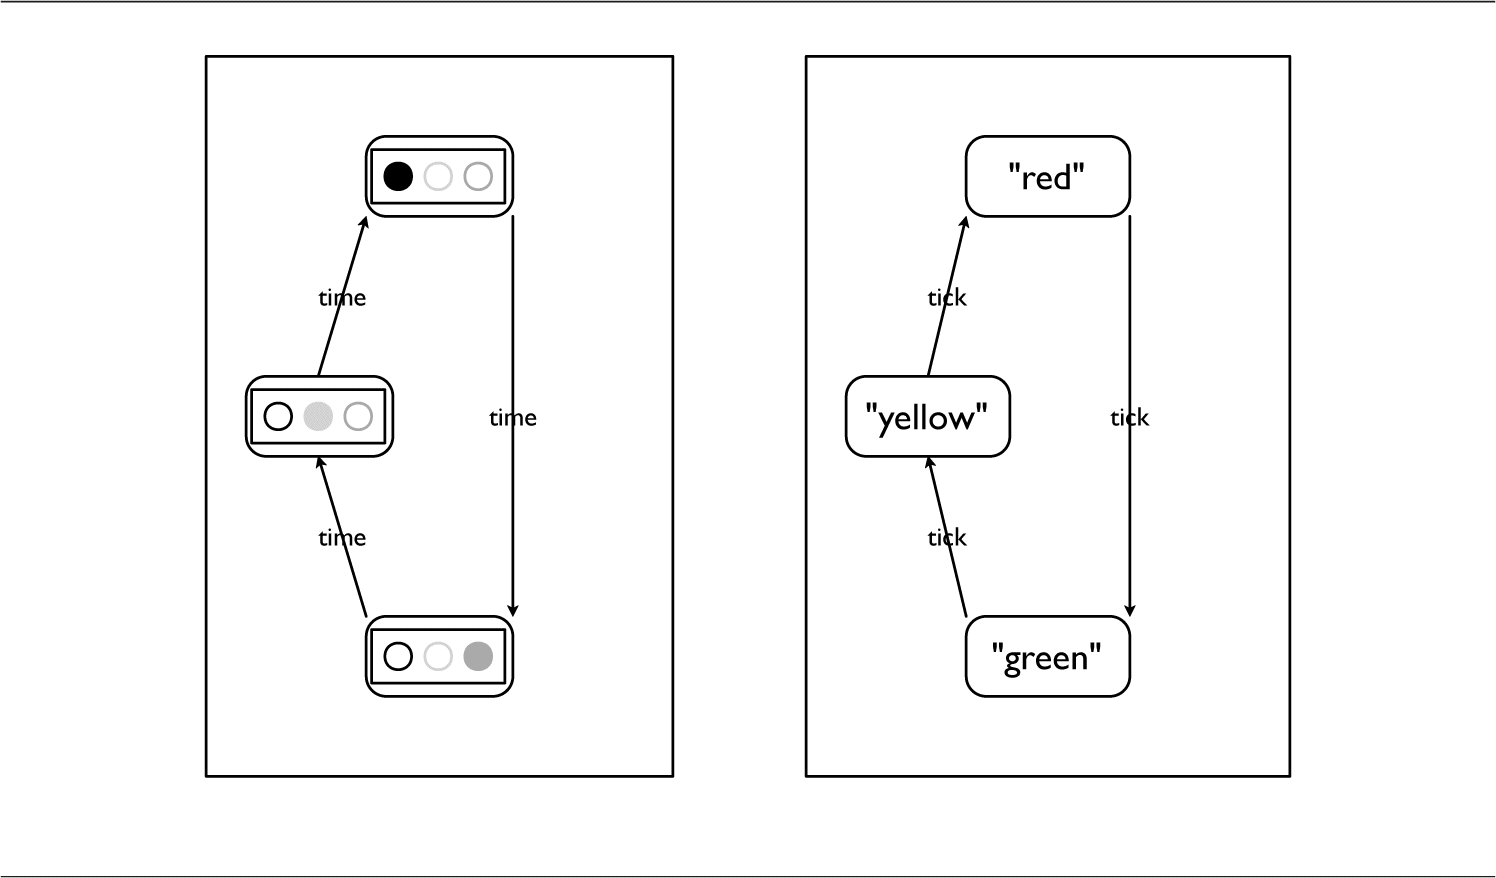
\includegraphics[width=0.7\textwidth]{images/00089.png}
  \caption{交通信号灯状态变迁图}
  \label{fig:traffic_light_fsa}
\end{figure}

图~\ref{fig:traffic_light_fsa} 显示了交通灯的状态变迁规律。每个状态由枚举定义，而状态跃迁函数 \code{tl-next} 则根据当前颜色决定下一颜色：

\begin{figure}[htbp]
  \centering
  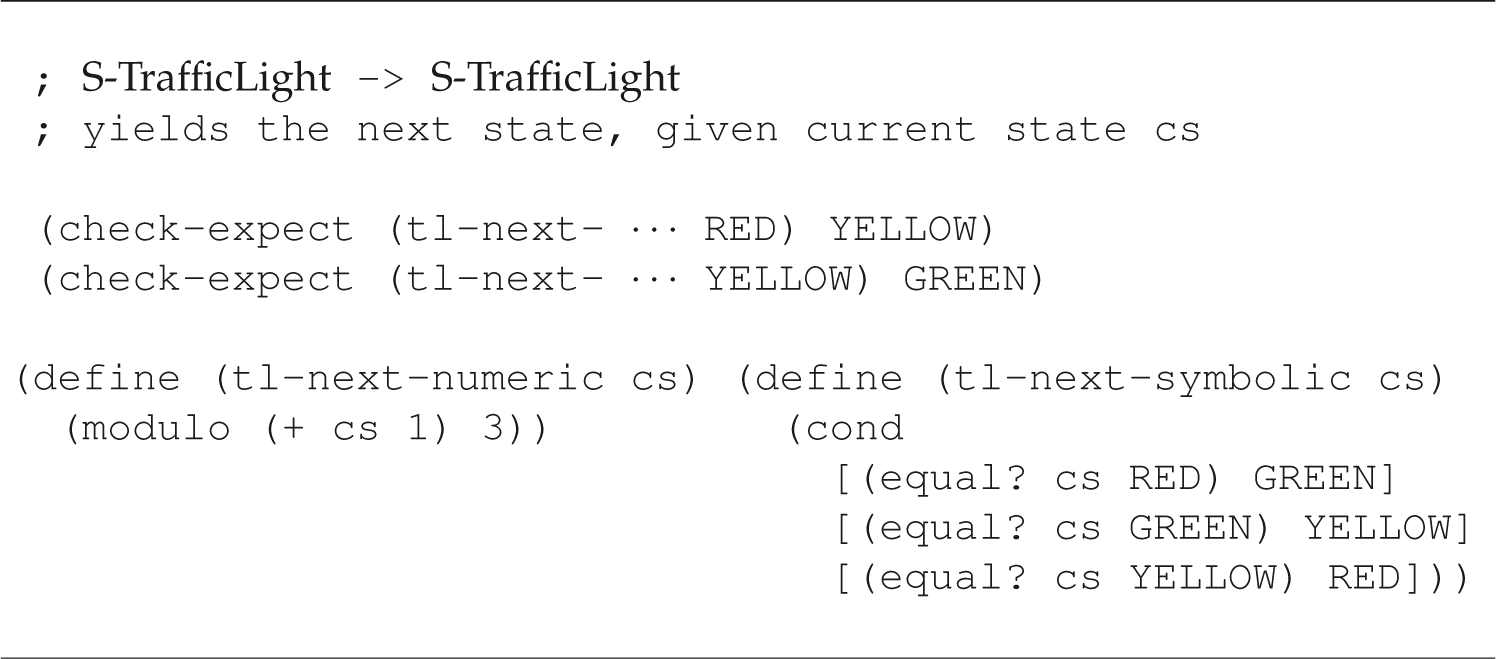
\includegraphics[width=0.85\textwidth]{images/00091.png}
  \caption{符号化交通信号灯程序定义}
  \label{fig:traffic_light_symbolic}
\end{figure}

\begin{exercise}{完善交通灯模拟程序}{59}
完成模拟交通灯状态机的世界程序设计，补全 \code{tl-render} 与 \code{tl-next} 的定义与全部测试。
\end{exercise}

\begin{exercise}{数值化交通灯状态}{60}
如果改用数值表示信号灯状态（0 表示红色，1 表示绿色，2 表示黄色），重构该程序并比较代码风格。
\end{exercise}

\begin{exercise}{使用符号常量}{61}
在数据定义与函数中使用符号常量（例如 \code{(define RED "red")}），消除程序中所有的“魔法字符串”。
\end{exercise}

\subsection{自动关门模拟程序}

考虑一个装有自动闭门器的安全防盗门。门具有三种状态：
\begin{itemize}
  \item \code{LOCKED}（已上锁）
  \item \code{CLOSED}（已关门但未上锁）
  \item \code{OPEN}（已开启）
\end{itemize}

\begin{figure}[htbp]
  \centering
  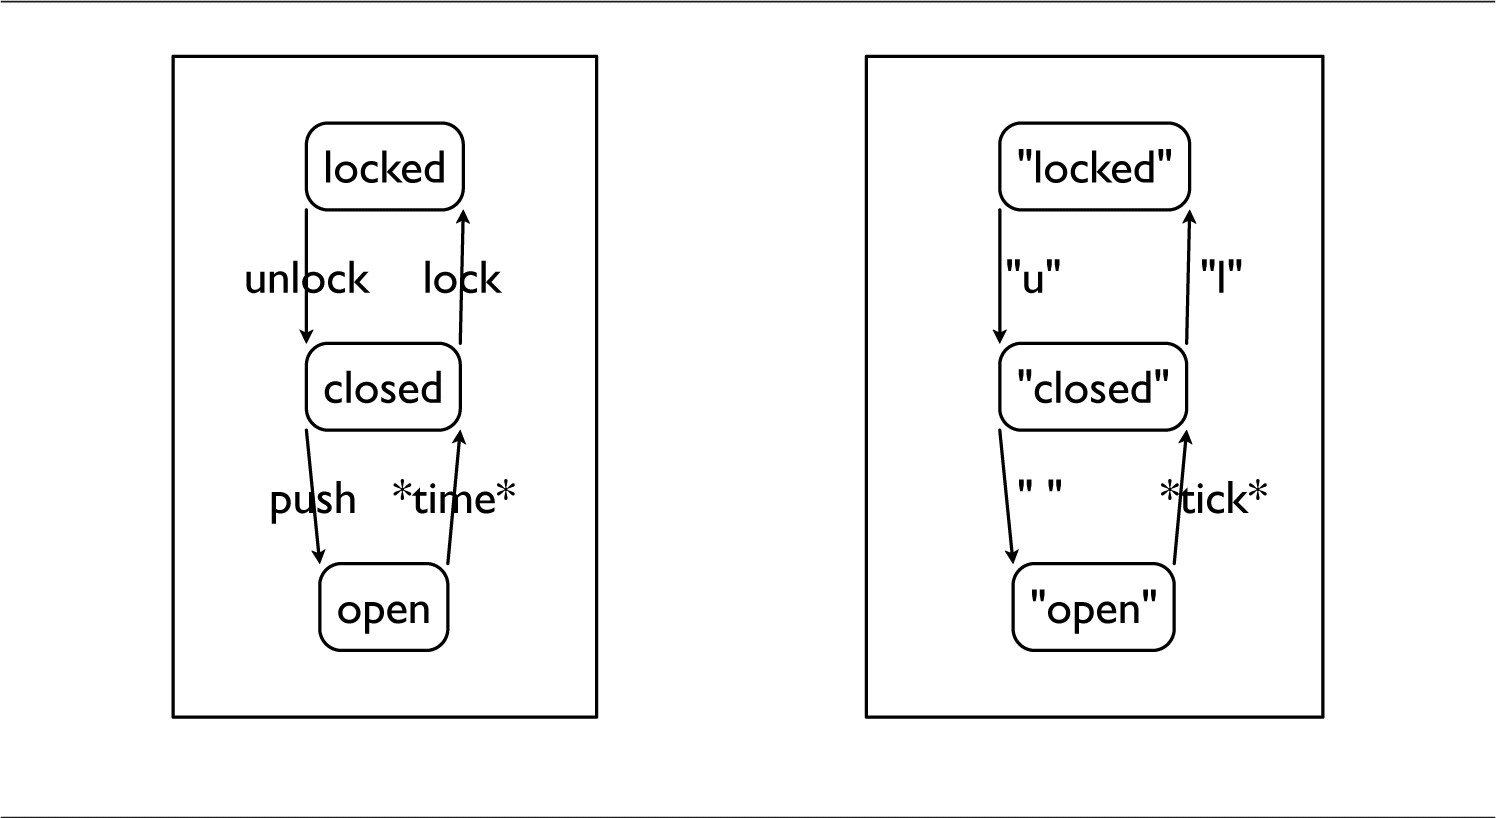
\includegraphics[width=0.75\textwidth]{images/00092.png}
  \caption{自动闭门防盗门的状态变迁图}
  \label{fig:door_fsa}
\end{figure}

如图~\ref{fig:door_fsa} 所示：
\begin{itemize}
  \item \textbf{时钟滴答（door-closer）}：自动闭门器在时钟滴答触发时将处于 \code{OPEN} 状态的门拉回 \code{CLOSED} 状态；其余状态保持不变。
  \item \textbf{按键操作（door-action）}：
    \begin{itemize}
      \item 当门处于 \code{LOCKED} 且按下 \code{"u"} 键时，门被解锁变为 \code{CLOSED}；
      \item 当门处于 \code{CLOSED} 且按下 \code{"l"} 键时，门被上锁变为 \code{LOCKED}；
      \item 当门处于 \code{CLOSED} 且按下空格键 \code{"\ "} 键时，门被推开变为 \code{OPEN}；
      \item 其余任何按键均不改变当前状态。
    \end{itemize}
\end{itemize}

我们可以将这两个函数的行为制成示例表格：

\begin{center}
\begin{tabular}{|l|l|}
\hline
\textbf{输入状态 (given state)} & \textbf{期望输出状态 (desired state)} \\
\hline
\code{LOCKED} & \code{LOCKED} \\
\code{CLOSED} & \code{CLOSED} \\
\code{OPEN}   & \code{CLOSED} \\
\hline
\end{tabular}
\end{center}

\begin{center}
\begin{tabular}{|l|l|l|}
\hline
\textbf{输入状态 (given state)} & \textbf{按键事件 (given key event)} & \textbf{期望输出状态 (desired state)} \\
\hline
\code{LOCKED} & \code{"u"} (unlock) & \code{CLOSED} \\
\code{CLOSED} & \code{"l"} (lock)   & \code{LOCKED} \\
\code{CLOSED} & \code{"\ "} (push)   & \code{OPEN} \\
\code{OPEN}   & 任意其他按键        & \code{OPEN} \\
\hline
\end{tabular}
\end{center}

\begin{figure}[htbp]
  \centering
  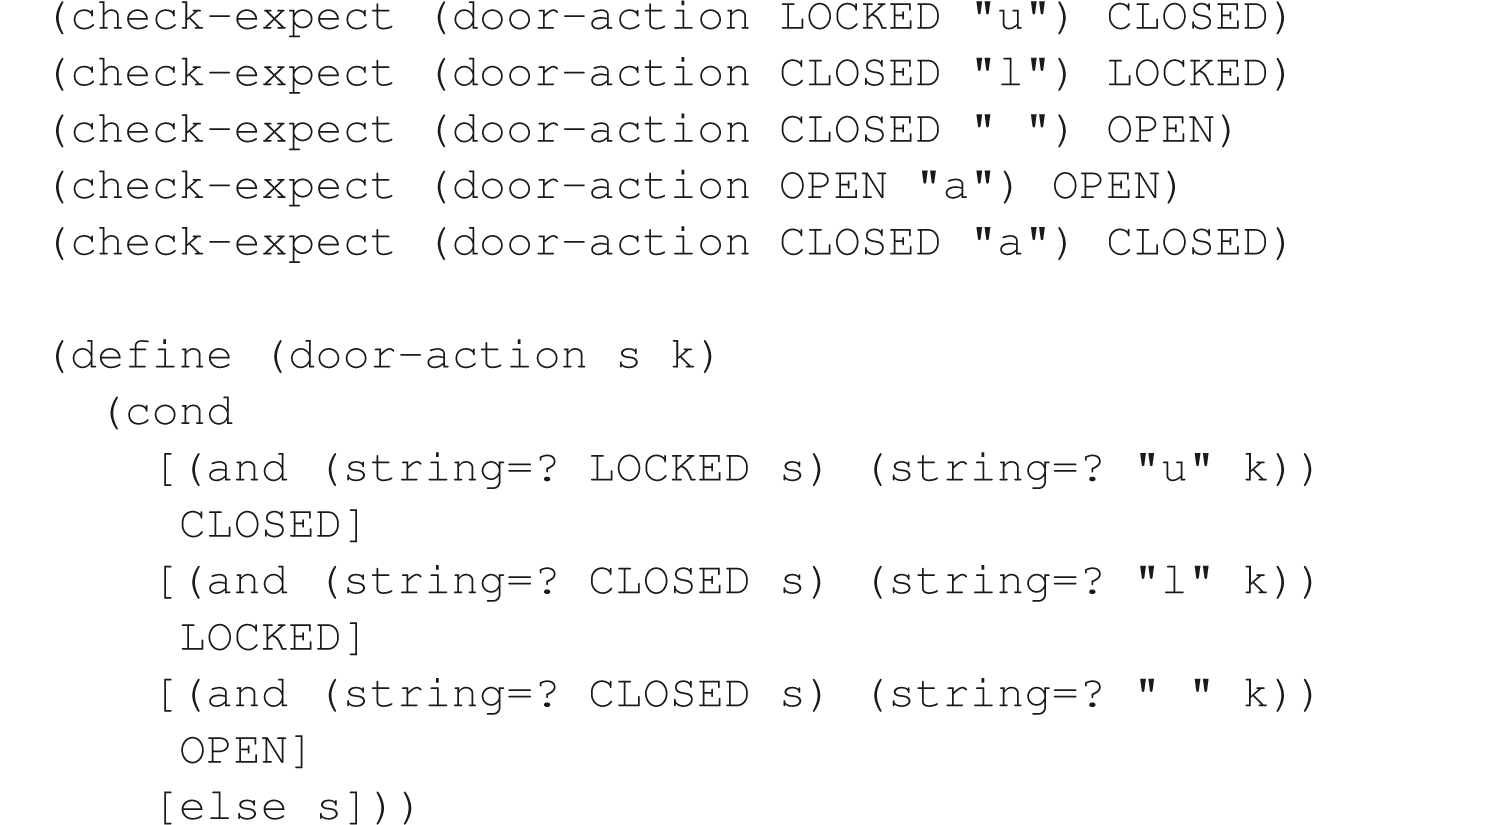
\includegraphics[width=0.85\textwidth]{images/00093.png}
  \caption{door-action 按键控制函数的实现与测试}
  \label{fig:door_closer_code}
\end{figure}

\begin{figure}[htbp]
  \centering
  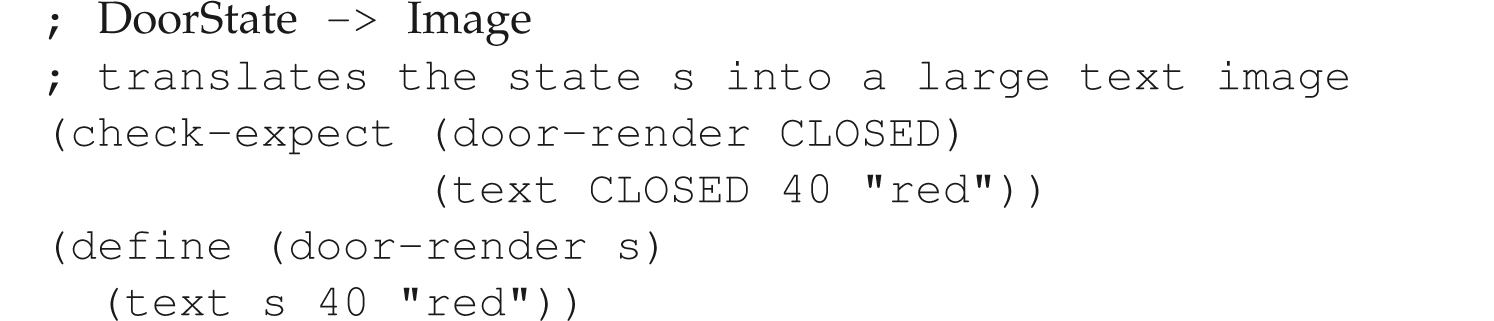
\includegraphics[width=0.85\textwidth]{images/00094.png}
  \caption{door-render 场景渲染函数的实现与测试}
  \label{fig:door_action_code}
\end{figure}

\begin{exercise}{调整仿真时钟速率}{62}
在运行防盗门模拟程序时，你可能会发现 \code{OPEN} 状态转瞬即逝（默认 1 秒有 28 个时钟滴答）。请修改 \code{door-simulation}，利用 \code{on-tick} 的时钟频率参数，使其每 3 秒才滴答一次，然后重新运行模拟并观察防盗门的开关动作。
\end{exercise}
